\documentclass{article}
\usepackage{geometry} 
\usepackage{TikZ}
\usepackage{relsize}
\geometry{paperwidth=1080pt, paperheight=1080pt}
\geometry{top=80pt, bottom=50pt, left=50pt, right=50pt}

\begin{document}
	

	
\begin{center}
	
	 \textscale{15}{\textbf{Geometric shape of DNA}}

		
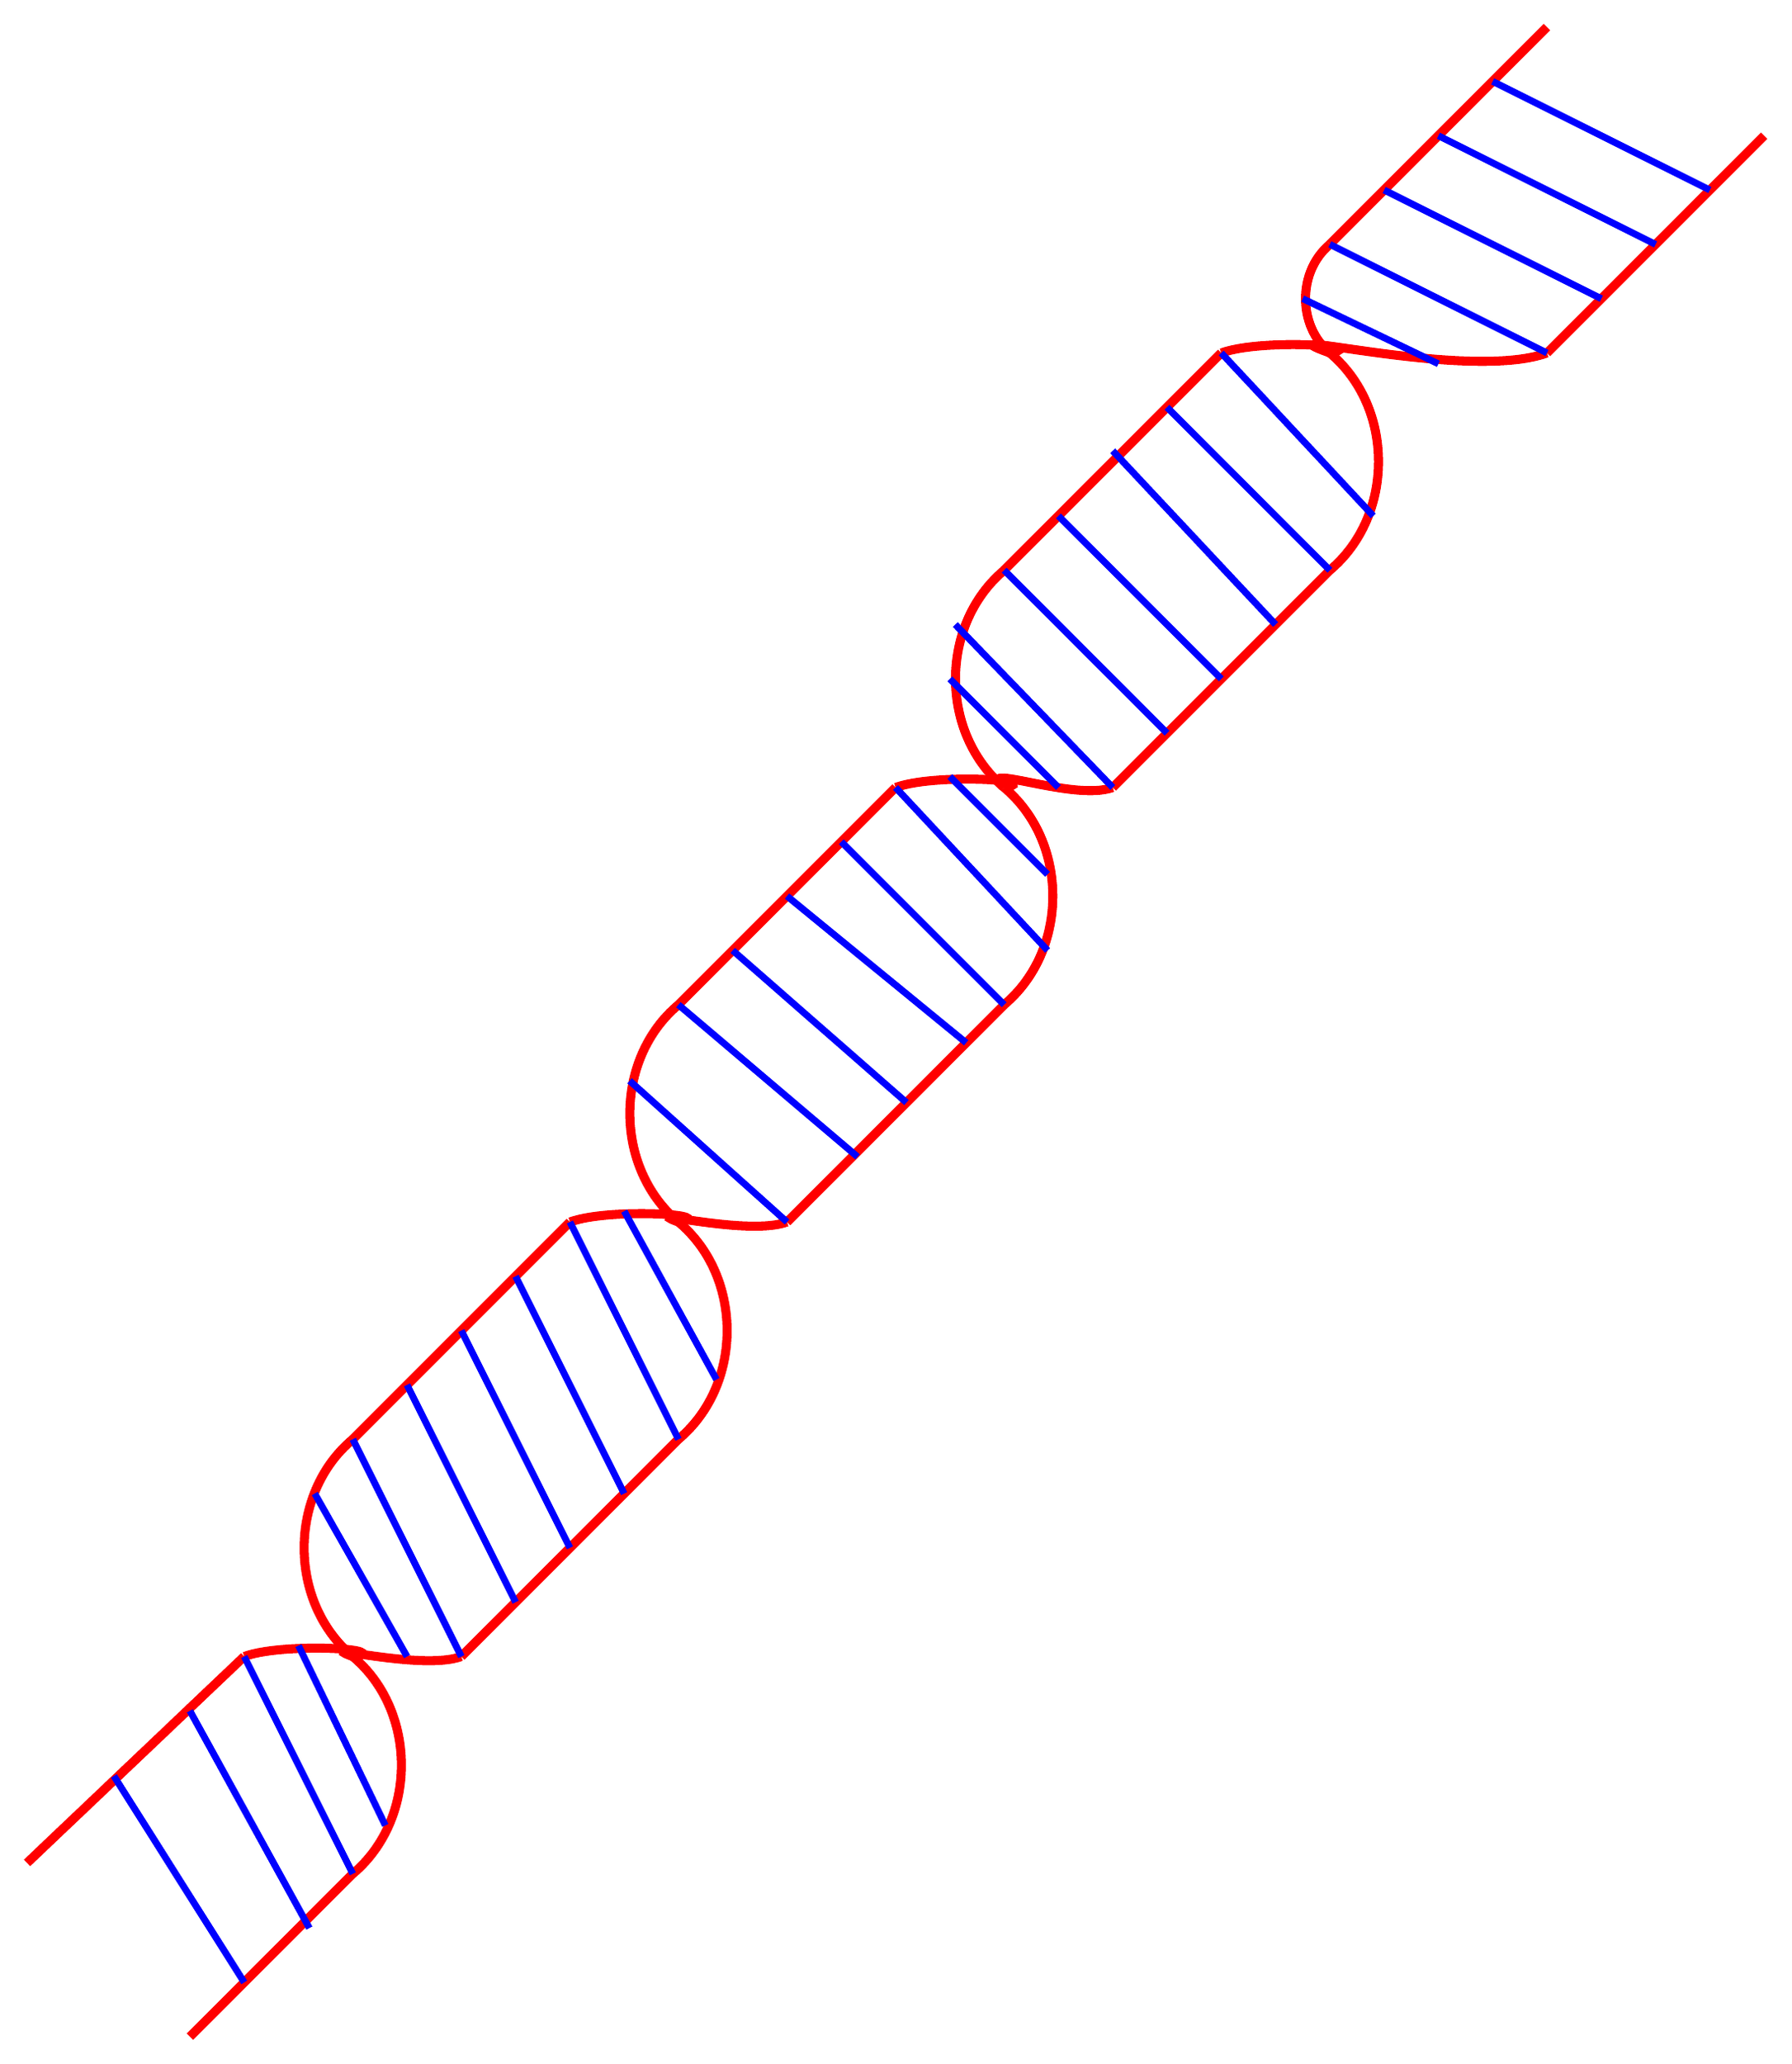
\begin{tikzpicture}[scale=1.69]
	
	
	
     \coordinate (A) at (6,9);
      \coordinate (B) at (8,8);
       \coordinate (C) at (4,7);
        \coordinate (D) at (6,6);
         \coordinate (E) at (4,6);
          \coordinate (F) at (3,6);
           \coordinate (G) at (4,4);
            \coordinate (H) at (1,4);
             \coordinate (I) at (2,2);
              \coordinate (J) at (1,2);
               \coordinate (K) at (0,2);
                \coordinate (L) at (1,0);
                 \coordinate (M) at (-2,0);
                  \coordinate (N) at (-1,-2);
                   \coordinate (O) at (-2,-2);
                    \coordinate (P) at (-3,-2);
                     \coordinate (Q) at (-2,-4);
                      \coordinate (R) at (-5,-4);
                       \coordinate (S) at (-4,-6);
                        \coordinate (T) at (-6,-6);
                         \coordinate (U) at (-5,-8);
                          \coordinate (V) at (-5,-6);
                           \coordinate (W) at (-8,-7.9);
                           \coordinate (X) at (-6.5,-9.5);
                           
      \coordinate (a) at (5.5,8.5); 
      \coordinate (b) at (7.5,7.5); 
      \coordinate (c) at (5,8); 
      \coordinate (d) at (7,7); 
      \coordinate (e) at (4.5,7.5); 
      \coordinate (f) at (6.5,6.5); 
      \coordinate (i) at (3.75,6.5); 
      \coordinate (j) at (5,5.9);     
      
      \coordinate (h) at (4.4,4.5); 
      \coordinate (g) at (2.5,5.5); 
      \coordinate (l) at (3.5,3.5); 
      \coordinate (k) at (2,5.1); 
      \coordinate (n) at (3,3); 
      \coordinate (m) at (1.5,4.5); 
      \coordinate (o) at (2.5,2.5); 
      \coordinate (p) at (0.55,3.5); 
      \coordinate (r) at (0.5,3); 
      \coordinate (s) at (1.5,2); 
      
      \coordinate (aa) at (0.5,2.1); 
      \coordinate (ak) at (1.4,1.2); 
      \coordinate (ac) at (-0.5,1.5); 
      \coordinate (ab) at (1.4,0.5); 
      \coordinate (ad) at (1,0); 
      \coordinate (ae) at (-1,1); 
      \coordinate (af) at (1.5,-0.5); 
      \coordinate (ag) at (-1.5,0.5);
      \coordinate (ah) at (0.1,-0.9); 
      \coordinate (ai) at (-0.35,-1.4); 
      \coordinate (aj) at (-2.45,-0.7); 
      \coordinate (al) at (-1,1); 
      \coordinate (am) at (0.65,-0.35);
      
      \coordinate (1) at (-2.5,-1.9); 
      \coordinate (2) at (-1.65,-3.45);     
      \coordinate (3) at (-3.5,-2.5);     
     \coordinate (4) at (-2.5,-4.5);
     \coordinate (5) at (-4,-3);     
     \coordinate (6) at (-3,-5);     
     \coordinate (7) at (-4.5,-3.5);     
     \coordinate (8) at (-3.5,-5.5);     
     \coordinate (9) at (-4.5,-6);    
     \coordinate (10) at (-5.35,-4.5);   
     \coordinate (11) at (-5.5,-5.9);     
     \coordinate (12) at (-4.7,-7.555);   
     \coordinate (13) at (-6.5,-6.5);     
     \coordinate (15) at (-7.2,-7.1);     
     \coordinate (16) at (-5.4,-8.5); 
     \coordinate (17) at (-6,-9);                     
      
                  
   
   \tikzset{every path/.style={line width=4pt, red}}
    \draw (A) -- (C);
    \draw (B) -- (D);
    \draw (F) -- (H);
    \draw (G) -- (I);
    \draw (K) -- (M);
    \draw (L) -- (N);
    \draw (P) -- (R);
    \draw (Q) -- (S);
    \draw (T) -- (W);
    \draw (U) -- (X);
    \draw (C) to[out=220,in=140] (E);
    \draw (D) to[out=200,in=160] (E);
    \draw (E) to[out=10,in=20] (F);
    \draw (E) to[out=-40,in=40] (G);
    \draw (H) to[out=220,in=140] (J);
    \draw (I) to[out=200,in=140] (J);
    \draw (J) to[out=10,in=20] (K);
    \draw (J) to[out=-40,in=40] (L);
    \draw (M) to[out=220,in=140] (O);
    \draw (N) to[out=200,in=160] (O);
    \draw (O) to[out=10,in=20] (P);
    \draw (O) to[out=-40,in=40] (Q);
    \draw (R) to[out=220,in=140] (V);
    \draw (S) to[out=200,in=160] (V);
    \draw (V) to[out=10,in=20] (T);
    \draw (V) to[out=-40,in=40] (U);
    
    \tikzset{every path/.style={line width=3pt, blue}}
    \draw (a) -- (b);
     \draw (c) -- (d);
      \draw (e) -- (f);
       \draw (C) -- (D);
        \draw (i) -- (j);
        
      \draw (F) -- (h);
       \draw (g) -- (G);
        \draw (k) -- (l);
         \draw (m) -- (n);
          \draw (H) -- (o);
           \draw (p) -- (I);
            \draw (r) -- (s);
        
         \draw (aa) -- (ak);
          \draw (K) -- (ab);
           \draw (ac) -- (ad);
            \draw (ae) -- (ae);
             \draw (ag) -- (ah);
              \draw (M) -- (ai);
               \draw (aj) -- (N);
                \draw (am) -- (al);  
                
     \draw (1) -- (2);
     \draw (P) -- (Q);
     \draw (3) -- (4);
     \draw (5) -- (6);
     \draw (7) -- (8);
     \draw (R) -- (S);
     \draw (10) -- (9);
     \draw (11) -- (12);
     \draw (T) -- (U);
     \draw (13) -- (16);
     \draw (15) -- (17);
       
    
    
    
   

    
\end{tikzpicture}

\#AEK

\end{center}


	 






\end{document}
